\section{Durchführung}
\label{sec:Durchführung}
Für den gesamten Versuch wird ein Lock-In-Verstärker mit eingbautem Vorverstärker, Tief- und Bandpass, Phasenverschieber,
sowie Funktions- und Rauschgenerator verwendet. Außerdem wird ein Oszilloskop

\begin{figure} [H]
    \centering
    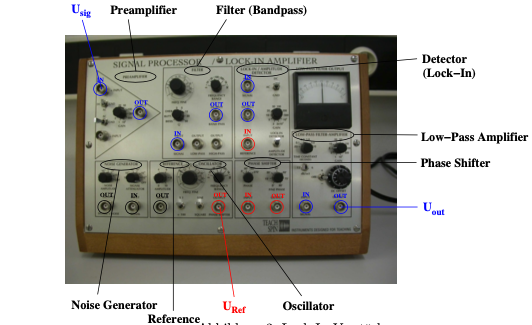
\includegraphics[height=8cm]{content/Bilder/Aufbau_Bild.png}
    \caption{Lock-In-Verstärker ohne Verkabelung.\cite{v303}}
    \label{fig:Aufbau Lock-In-Verstaerker}
\end{figure}
